%% CAIRN manuscript — Springer Nature sn-jnl, sn-mathphys-num style.
%% Build: pdflatex main && bibtex main && pdflatex main && pdflatex main
%% Anonymity: flip \anontrue / \anonfalse below.

\documentclass[pdflatex,sn-mathphys-num]{sn-jnl}

\usepackage{graphicx}
\usepackage{amsmath,amssymb,amsthm}
\usepackage{booktabs}
\usepackage{algorithm}
\usepackage{algpseudocode}
\usepackage{tikz}
\usetikzlibrary{arrows.meta,positioning,fit,calc}

\newif\ifanon
\anontrue % review version; set \anonfalse for the camera-ready copy

\theoremstyle{thmstyleone}
\newtheorem{proposition}{Proposition}
\newtheorem{lemma}{Lemma}
\theoremstyle{thmstylethree}
\newtheorem{assumption}{Assumption}
\newtheorem{remark}{Remark}

\newcommand{\dt}{\mathrm{do}}
\newcommand{\E}{\mathbb{E}}
\renewcommand{\Pr}{\mathbb{P}}
\newcommand{\Lpin}{\mathcal{L}^{\mathrm{pin}}}
\newcommand{\Lint}{\mathcal{L}^{\mathrm{int}}}
\newcommand{\Linv}{\mathcal{L}^{\mathrm{inv}}}
\newcommand{\Lcal}{\mathcal{L}^{\mathrm{cal}}}

\raggedbottom

\begin{document}

\title[CAIRN: A Causally-Factored, Self-Certifying World Model]{CAIRN: A causally-factored, self-certifying world model for interventional generalization}

\ifanon
\author*[1]{\fnm{Anonymous} \sur{Author}}\email{anonymous@review.org}
\affil*[1]{\orgname{Anonymous Institution}}
\else
\author*[1]{\fnm{Quang-Vinh} \sur{Dang}}\email{vinh.dq4@buv.edu.vn}
\affil*[1]{\orgname{British University Vietnam}, \orgaddress{\city{Hung Yen}, \country{Vietnam}}}
\fi

\abstract{State-of-the-art world models learn a monolithic transition map
in which every latent variable depends on every other and actions
condition the entire map at once. Because of this structural commitment,
a change to a single mechanism of the environment---a damaged actuator, an
altered friction coefficient, a failing financial protocol---renders the
whole learned model off-support: the model can neither localize the change
nor adapt to it, and it fails silently. We introduce CAIRN (Causal
Action-conditioned Interventional Rollout Network), a world-model
architecture and training algorithm in which (i) latent dynamics factor
over a learned sparse causal graph, (ii) actions and exogenous shocks
enter as interventions on specific mechanisms in the sense of Pearl's
do-operator, implemented architecturally as graph surgery, and (iii) every
mechanism carries an internal betting martingale---the \emph{e-gate}---so
that the model maintains anytime-valid statistical evidence about which
parts of itself are currently wrong. The e-gate drives three capabilities
that a monolithic model cannot offer: evidence-triggered localized
adaptation that refits only the broken mechanism, evidence-proportional
uncertainty inflation that widens predictive intervals for exactly the
variables a stale mechanism generates, and online repair of the causal
graph itself. We prove that each gate controls its false-alarm probability
uniformly over time under a composite null that absorbs the quantile
approximation error of learned mechanisms, and we bound its detection
delay. On a ground-truth causal benchmark, CAIRN detects unannounced
single-mechanism shifts within a median of eighteen steps at a measured
false-alarm rate of zero, localizes the shifted mechanism with an $F_1$ of
$0.97$ where an oracle-tuned CUSUM reaches $0.68$ and ensemble
disagreement $0.28$, adapts without any interference on healthy
mechanisms where full fine-tuning catastrophically degrades them, and
keeps rollout intervals calibrated before, during, and after the shift.}

\keywords{world models, causal representation learning, anytime-valid
inference, e-processes, distribution shift, model-based reinforcement
learning}

\maketitle

\section{Introduction}\label{sec:intro}

A world model is a learned simulator that an agent carries inside itself:
given the current state and a candidate course of action, it imagines how
the future unfolds, and the agent plans against those imagined futures
rather than against the far more expensive real world
\citep{ha2018world,hafner2025mastering,hansen2024tdmpc2}. The past years
have produced world models of remarkable breadth, from recurrent
state-space models that support control purely from imagination
\citep{hafner2025mastering} to latent-dynamics models embedded in
model-predictive control \citep{hansen2024tdmpc2}, autoregressive
token-based dynamics \citep{micheli2023transformers}, and generative video
models that render entire interactive environments
\citep{bruce2024genie}. Despite their diversity, these models share one
structural commitment: the transition function is a \emph{monolithic map}
$\hat{s}_{t+1}=f_\theta(s_t,a_t)$ in which every latent dimension depends
on every other and the action conditions the whole map.

Because of this commitment, three well-documented failure modes follow.
First, the models are \emph{interventionally brittle}: when one mechanism
of the environment changes---an object's mass, a joint's gain, the
collateral rule of one financial protocol---the entire learned transition
is off-support, so the model cannot localize the change, cannot adapt to
it without retraining everything, and its rollouts degrade globally even
though most of the world is unchanged. Second, they carry \emph{no native
validity semantics}: a monolithic model emits point predictions or
heuristic ensemble variances \citep{chua2018deep}, but nothing inside it
can state, with controlled error, that a particular part of its dynamics
is currently stale. Third, \emph{actions are not treated as
interventions}: physically and economically an action manipulates specific
variables and its effects propagate through structure, yet conditioning a
monolithic map on the action vector discards exactly the sparsity that
compositional generalization to unseen action--state combinations
requires \citep{scholkopf2021toward,pearl2009causality}.

Recent causal world-model research addresses the third point by factoring
the transition over a learned causal graph
\citep{wang2022causal,wang2022denoised}, and interventional causal
representation learning provides identifiability foundations for such
factorizations \citep{ahuja2023interventional}. What remains missing is
any mechanism by which the model itself \emph{notices}, during deployment
and with statistical guarantees, that one of its mechanisms has become
invalid---and then responds locally rather than globally. Post-hoc
monitoring wrappers such as adaptive conformal inference
\citep{gibbs2021adaptive} and online randomness testing
\citep{vovk2021testing} operate outside the model on scalar summaries;
they can raise a global alarm but cannot say \emph{which} mechanism broke,
let alone repair it.

This paper closes that gap with CAIRN, a world model whose central design
principle is that \emph{the causal factorization and the validity
monitoring must be built together}, because each is what makes the other
useful. The factorization gives every latent variable its own small
mechanism with a sparse parent set; the monitoring equips every mechanism
with an internal betting martingale over its own predictive validity, in
the tradition of game-theoretic statistics
\citep{shafer2019game,ramdas2023game,waudbysmith2024estimating}. When a
mechanism is valid, no betting strategy can grow wealth systematically;
when it breaks, wealth grows exponentially, and by Ville's inequality
\citep{ville1939etude} the wealth crossing a threshold $1/\delta$ is an
anytime-valid, per-mechanism alarm at level $\delta$ that requires no
tuning and no multiple-testing correction over continuous monitoring.
Because the alarm names a specific mechanism, the response can be local:
spawn a fresh copy of that mechanism, refit it on a short recent window,
and leave the rest of the model untouched; persistent alarms after refit
indicate a wrong parent set and trigger a local re-search of the graph.

Our contributions are as follows. First, we specify the CAIRN model class
and training objective: a transition kernel factored over a learned
adjacency and a learned action-target mask, distributional (quantile)
mechanism heads, interventions as architectural graph surgery, and a joint
loss combining quantile regression, sparsity, interventional consistency,
a sparse-mechanism-shift invariance penalty, and a differentiable rollout
calibration term (Section~\ref{sec:method}). Second, we develop the
e-gate: a composite betting e-process over probability-integral-transform
residuals with Online Newton Step bet sizing, a conformal recalibration
step that restores finite-sample validity under learned quantile heads,
and a \emph{tolerance null} that keeps Ville's guarantee exact in the
presence of irreducible approximation error; we prove time-uniform
false-alarm control, bound detection delay, and give conditions under
which alarms localize to the truly shifted mechanisms
(Section~\ref{sec:egate}). Third, we show how the gate's wealth acts
inside the model: evidence-weighted mechanism mixtures, uncertainty
inflation, and online structure repair, together with risk-sensitive
planning through quantile rollouts (Section~\ref{sec:deploy}). Fourth, on
a ground-truth synthetic benchmark with scriptable mechanism shifts we
evaluate six pre-registered research questions against monolithic,
ensemble, and change-detection baselines, reporting both the successes
and the places where the causal machinery does not help
(Section~\ref{sec:experiments}).

\section{Related work}\label{sec:related}

\paragraph{World models.} Learned latent dynamics for planning date back
at least to the recurrent world models of \citet{ha2018world}; the
Dreamer line established imagination-based actor--critic learning at
scale, culminating in a single configuration that masters diverse control
domains \citep{hafner2025mastering}. TD-MPC2 couples latent dynamics with
sampling-based model-predictive control \citep{hansen2024tdmpc2}, IRIS
treats dynamics as autoregressive token prediction
\citep{micheli2023transformers}, and Genie generates playable
environments from video alone \citep{bruce2024genie}. Probabilistic
ensembles quantify epistemic uncertainty by disagreement
\citep{chua2018deep}. All of these share the monolithic transition map
whose failure under localized change motivates our work.

\paragraph{Causal dynamics and representations.} Factoring dynamics along
causal structure is the program of causal representation learning
\citep{scholkopf2021toward}. Causal dynamics learning recovers sparse
transition structure for state abstraction \citep{wang2022causal}, and
Denoised MDPs separate controllable from uncontrollable factors
\citep{wang2022denoised}. Identifiability of latent causal variables from
interventional data is analyzed by \citet{ahuja2023interventional}.
Differentiable structure learning descends from NOTEARS
\citep{zheng2018dags}; in our temporal setting edges run strictly forward
in time, so the acyclicity constraint---the least stable ingredient of
that line---is unnecessary. CausalWorld provides a robotic benchmark with
ground-truth causal structure \citep{ahmed2021causalworld}; our synthetic
suite plays the same role at smaller scale with exact scoring. None of
these systems monitor their own mechanisms' validity online.

\paragraph{Anytime-valid monitoring.} Testing by betting goes back to
\citet{ville1939etude} and has been developed into a general theory of
safe, anytime-valid inference
\citep{shafer2019game,ramdas2023game,waudbysmith2024estimating}. Online
randomness testing with conformal martingales \citep{vovk2021testing} and
adaptive conformal inference \citep{gibbs2021adaptive} monitor a model
from the outside. CAIRN internalizes the martingale: one e-process per
mechanism, whose wealth feeds back into prediction, adaptation, and
structure repair. Our bet sizing uses Online Newton Step, whose
logarithmic regret for exp-concave losses \citep{hazan2007logarithmic}
underlies the detection-delay bound. Calibration of distributional
forecasts via the probability integral transform is classical
\citep{gneiting2007probabilistic}, as is quantile regression via the
pinball loss \citep{koenker1978regression}.

\section{The CAIRN world model}\label{sec:method}

\subsection{Model class}\label{sec:model}

An encoder $q_\phi$ maps observations to a latent state partitioned into
$d$ variables $z_t=(z_t^1,\dots,z_t^d)$. In the state-space instantiation
studied experimentally the partition is given and the encoder is the
identity; in pixel instantiations a frozen visual encoder such as DINOv2
\citep{oquab2024dinov2} supplies the latent stream, and everything
downstream is unchanged. Structure is carried by two learned binary
matrices: an adjacency $A\in\{0,1\}^{d\times d}$, where $A_{ji}=1$ means
$z^j_t$ is a parent of $z^i_{t+1}$, and an action-target mask
$M\in\{0,1\}^{m\times d}$, where $M_{ki}=1$ means action coordinate $k$
acts on variable $i$. Both are parameterized by Gumbel-sigmoid
relaxations with straight-through gradients
\citep{jang2017categorical,maddison2017concrete}. Because edges run from
$t$ to $t{+}1$, the graph is a dynamic Bayesian network and no acyclicity
penalty is needed.

The transition kernel factorizes over mechanisms,
\begin{equation}\label{eq:factored}
p_\theta\bigl(z_{t+1}\mid z_t,a_t\bigr)
 \;=\;\prod_{i=1}^{d}
 p_{\theta_i}\!\bigl(z^i_{t+1}\mid z_t\odot A_{\cdot i},\;
 a_t\odot M_{\cdot i}\bigr),
\end{equation}
where each mechanism $f_i$ is a small multilayer perceptron whose input
is masked elementwise by its parent and target columns, so structure
gradients flow through the masks. Every mechanism carries a
\emph{distributional head}: it outputs a vector of $K$ quantiles
$\{\hat{z}^i_{t+1}(\tau_k)\}_{k=1}^{K}$ at fixed levels
$\tau_1<\dots<\tau_K$, made non-crossing by accumulating
softplus-positive increments, and trained with the pinball loss
\citep{koenker1978regression}
\begin{equation}\label{eq:pinball}
\Lpin_i \;=\; \frac{1}{K}\sum_{k=1}^{K}
\rho_{\tau_k}\!\bigl(z^i_{t+1}-\hat{z}^i_{t+1}(\tau_k)\bigr),
\qquad
\rho_\tau(u)=\max\{\tau u,\,(\tau-1)u\}.
\end{equation}
Rollouts propagate samples drawn by inverting the piecewise-linear
quantile function, so imagination is a distribution over trajectories and
predictive intervals at every horizon come for free.

Interventions are first-class inputs. An intervention
$\dt(z^i{\leftarrow}v)$---an agent action reaching variable $i$ through
$M$, or an exogenous labeled shock---\emph{replaces} mechanism $i$'s
output by the substituted value rather than conditioning it. This is the
graph-surgery semantics of the do-operator \citep{pearl2009causality}
implemented architecturally: parents severed, value substituted.
Counterfactual rollouts are therefore a forward pass. A direct
consequence, used repeatedly below, is that variables that are not
descendants of the intervened node are provably untouched by the
intervention in the model's imagination
(Figure~\ref{fig:surgery}).

\begin{figure}[t]
\centering
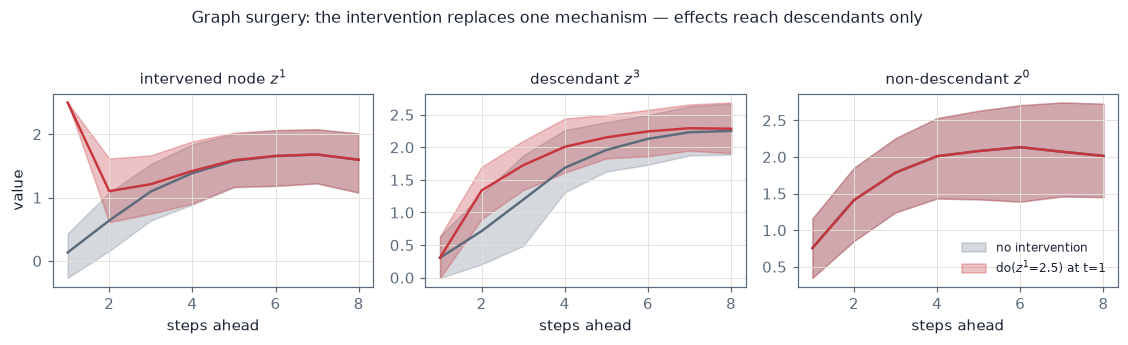
\includegraphics[width=\textwidth]{figures/fig_surgery.png}
\caption{Graph surgery in imagination on the ground-truth benchmark of
Section~\ref{sec:experiments}. The query $\dt(z^1{=}2.5)$ pins the
intervened variable at the surgery step (left), shifts the distribution of
its descendant (middle), and leaves the non-descendant's imagined future
exactly unchanged---the intervention band coincides with the
no-intervention band (right). A monolithic model cannot make this
promise.}\label{fig:surgery}
\end{figure}

\subsection{The e-gate}\label{sec:egate}

The e-gate converts each observed transition into evidence about each
mechanism's validity. Let $F^i_t$ denote the predictive distribution that
mechanism $i$ stated for $z^i_{t+1}$ (the piecewise-linear distribution
through its quantiles), and let
\begin{equation}\label{eq:pit}
u^i_t \;=\; F^i_t\bigl(z^i_{t+1}\bigr)\in(0,1)
\end{equation}
be the (randomized-tail) probability integral transform of the realized
value. If the stated distribution is the true conditional law, then
$u^i_t$ is uniform on $(0,1)$ conditionally on the past
\citep{gneiting2007probabilistic}. Mechanism $i$ bets against this
uniformity with a wealth process
\begin{equation}\label{eq:wealth}
W^i_t \;=\; \prod_{s\le t}\Bigl(1+\lambda^i_s\,
\bigl(g(u^i_s)-\varepsilon\,\mathrm{sign}\,\lambda^i_s\bigr)\Bigr),
\qquad W^i_0=1,
\end{equation}
where $g$ is a bounded payoff with $\E[g(U)]=0$ under uniformity,
$\lambda^i_s\in[-\tfrac12,\tfrac12]$ is a predictable bet, and
$\varepsilon\ge 0$ is a tolerance whose role is explained below. We run
two elementary payoffs per gate, a location bet $g_1(u)=2u-1$ and a
dispersion bet $g_2(u)=6(u-\tfrac12)^2-\tfrac12$, both bounded in
$[-1,1]$, and combine the two wealth processes by averaging, which
preserves the e-process property. Bets are sized by Online Newton Step on
the log-wealth,
\begin{equation}\label{eq:ons}
\lambda_{t+1} \;=\;
\Pi_{[-\frac12,\frac12]}\!\Bigl(\lambda_t+\tfrac{2}{2-\ln 3}\,
\tfrac{\nabla_t}{\sum_{s\le t}\nabla_s^2}\Bigr),
\qquad
\nabla_t=\frac{g(u_t)-\varepsilon\,\mathrm{sign}\,\lambda_t}
{1+\lambda_t(g(u_t)-\varepsilon\,\mathrm{sign}\,\lambda_t)},
\end{equation}
following \citet{waudbysmith2024estimating}. The gate \emph{alarms} the
first time $W^i_t\ge 1/\delta$.

Two practical refinements make the guarantee hold for \emph{learned}
mechanisms rather than only for ideal ones. First, before deployment the
raw PIT values are passed through a conformal recalibration map fitted on
held-out data---the randomized empirical distribution function of
calibration PITs---which makes the deployed PITs exactly uniform under
exchangeability with the calibration set regardless of quantile-head
bias; the same sliding-holdout recalibration runs periodically during
deployment for gate-quiet mechanisms. Second, the tolerance
$\varepsilon>0$ in \eqref{eq:wealth} converts the null from exact
uniformity to the composite null ``approximately valid'', which is the
operationally correct null when mechanisms carry irreducible
approximation error: a learned model that is wrong by a hair should not
be flagged as broken, while a mechanism whose physics changed produces
payoffs far outside the tolerance and is caught within tens of steps.

\begin{proposition}[Anytime-valid false-alarm control]
\label{prop:validity}
Fix $\delta\in(0,1)$ and $\varepsilon\ge 0$, and let
$(u_t)_{t\ge1}$ be any sequence adapted to a filtration
$(\mathcal{F}_t)$ such that
$\bigl|\E[g(u_t)\mid\mathcal{F}_{t-1}]\bigr|\le\varepsilon$ for all $t$.
Then the wealth \eqref{eq:wealth} with any predictable bets
$\lambda_t\in[-\tfrac12,\tfrac12]$ satisfies
$\Pr\bigl(\exists t:\,W_t\ge 1/\delta\bigr)\le\delta$.
\end{proposition}

\begin{proof}
Write $Y_t=\lambda_t\bigl(g(u_t)-\varepsilon\,\mathrm{sign}\,
\lambda_t\bigr)$. Since $\lambda_t$ is $\mathcal{F}_{t-1}$-measurable,
\[
\E[Y_t\mid\mathcal{F}_{t-1}]
=\lambda_t\,\E[g(u_t)\mid\mathcal{F}_{t-1}]
-\varepsilon\lvert\lambda_t\rvert
\;\le\;\lvert\lambda_t\rvert\bigl(\bigl|\E[g(u_t)\mid
\mathcal{F}_{t-1}]\bigr|-\varepsilon\bigr)\;\le\;0 .
\]
Moreover $Y_t\ge-\tfrac12(1+\varepsilon)>-1$, so $1+Y_t>0$ and
$\E[1+Y_t\mid\mathcal{F}_{t-1}]\le 1$; hence
$W_t=\prod_{s\le t}(1+Y_s)$ is a nonnegative supermartingale with
$W_0=1$. Ville's inequality \citep{ville1939etude} gives
$\Pr(\sup_t W_t\ge 1/\delta)\le\delta$. The average of the two payoffs'
wealth processes is again a nonnegative supermartingale with initial
value one, so the composite gate inherits the same bound.
\end{proof}

\begin{proposition}[Detection delay]\label{prop:delay}
Suppose that after an unannounced change the payoffs are independent and
identically distributed with $\mu=\E[g(u_t)]$ satisfying
$\lvert\mu\rvert>\varepsilon$. Let
$r=\dfrac{(\lvert\mu\rvert-\varepsilon)^2}{4(1+\varepsilon)^2}$. Then the
gate with the fixed oracle bet
$\lambda^\ast=\mathrm{sign}(\mu)\,
\dfrac{\lvert\mu\rvert-\varepsilon}{2(1+\varepsilon)^2}$ satisfies
$\liminf_{t\to\infty}\tfrac1t\log W_t\ge r$ almost surely, so its alarm
time is at most $(1+o(1))\log(1/\delta)/r$; and the ONS gate
\eqref{eq:ons} attains the same asymptotic rate, since its log-wealth is
within $O(\log t)$ of the best constant bet in hindsight.
\end{proposition}

\begin{proof}
Set $s=\mathrm{sign}(\mu)$ and $Y_t=\lambda^\ast(g(u_t)-\varepsilon s)$.
Then $\lvert Y_t\rvert\le\lvert\lambda^\ast\rvert(1+\varepsilon)\le
\tfrac12$, and for $\lvert y\rvert\le\tfrac12$ one has
$\log(1+y)\ge y-y^2$. Hence
\[
\E\log(1+Y_t)\;\ge\;\E Y_t-\E Y_t^2
\;\ge\;\lvert\lambda^\ast\rvert(\lvert\mu\rvert-\varepsilon)
-\lvert\lambda^\ast\rvert^2(1+\varepsilon)^2
\;=\;r,
\]
where the last equality follows by substituting $\lambda^\ast$. By the
strong law of large numbers applied to the i.i.d.\ bounded variables
$\log(1+Y_t)$, $\tfrac1t\log W_t(\lambda^\ast)\to\E\log(1+Y_1)\ge r$
almost surely, and $W_t\ge 1/\delta$ once
$t\ge(1+o(1))\log(1/\delta)/r$. The losses
$-\log(1+\lambda(g_t-\varepsilon\,\mathrm{sign}\lambda))$ are exp-concave
in $\lambda$ on the compact bet space, so Online Newton Step guarantees
$\log W_t(\text{ONS})\ge\log W_t(\lambda^\ast)-O(\log t)$
\citep{hazan2007logarithmic}, which does not affect the leading term.
\end{proof}

\begin{proposition}[Localization]\label{prop:local}
Consider a shift confined to a mechanism subset $S$, and suppose that for
every $i\notin S$ the stated predictive distribution of mechanism $i$
remains within the betting tolerance, in the sense that
$\bigl|\E[g_k(u^i_t)\mid\mathcal{F}_{t-1}]\bigr|\le\varepsilon$ for both
payoffs and all $t$. Then every gate outside $S$ alarms with probability
at most $\delta$ over the entire deployment, while every gate $i\in S$
whose post-change payoff mean exceeds the tolerance by
$\Delta_i=\lvert\mu_i\rvert-\varepsilon>0$ alarms within
$(1+o(1))\,4(1+\varepsilon)^2\log(1/\delta)/\Delta_i^2$ steps. Family-wise
control over the $d-\lvert S\rvert$ healthy gates holds at level
$(d-\lvert S\rvert)\delta$ by the union bound, or at level $\delta$ by
merging the per-gate e-values by averaging.
\end{proposition}

\begin{proof}
The monitoring inputs of gate $i$ are functions of the \emph{realized}
transition $(z_t,a_t,z^i_{t+1})$ only: predictions are conditioned on the
observed state, never on imagined values. A shift of the mechanisms in
$S$ changes the law of $z^j_{t+1}$ for $j\in S$ and, through the state,
the distribution of \emph{inputs} visited by other mechanisms; but the
conditional law of $z^i_{t+1}$ given $(z_t,a_t)$ for $i\notin S$ is
unchanged, and by hypothesis the stated distribution remains within
tolerance on the visited inputs. Proposition~\ref{prop:validity} then
applies to each healthy gate separately, giving the per-gate bound; the
union bound and the fact that an average of e-values is an e-value give
the two family-wise statements. The delay claim is
Proposition~\ref{prop:delay} applied to each $i\in S$.
\end{proof}

\begin{remark}
The hypothesis of Proposition~\ref{prop:local} is exactly where honest
caveats live: a healthy mechanism can leave its tolerance when the
shifted state distribution drives it into input regions where its
approximation error is larger than $\varepsilon$. Empirically
(Section~\ref{sec:rq2}) this collateral effect is rare and mild, and the
periodic recalibration of gate-quiet mechanisms absorbs slow drifts of
this kind, at the documented price that sub-tolerance drifts are
absorbed rather than flagged.
\end{remark}

\subsection{Training objective}\label{sec:training}

CAIRN is trained on trajectory data spanning multiple regimes
$e\in\mathcal{E}$, each regime differing from the nominal one by a sparse
mechanism shift, together with a fraction of steps carrying labeled
do-interventions. The loss combines five terms,
\begin{equation}\label{eq:loss}
\mathcal{L}
=\sum_{i=1}^d \Lpin_i
+\gamma_1\bigl(\lVert A\rVert_1+\lVert M\rVert_1\bigr)
+\gamma_2\,\Lint
+\gamma_3\,\Linv
+\gamma_4\,\Lcal ,
\end{equation}
whose parts we describe in turn. The pinball term $\Lpin$ is the
teacher-forced one-step loss \eqref{eq:pinball} plus a multi-step
latent-overshooting variant in which the predicted median is propagated
through short segments and penalized at every step, fighting compounding
error. The sparsity term applies an $\ell_1$ penalty to the edge and
target probabilities. The interventional-consistency term $\Lint$ applies
the same multi-step pinball loss on segments containing labeled
interventions, computed through the do-surgery forward pass, so that both
$A$ and $M$ receive interventional rather than merely observational
signal---the ingredient that identifiability results require
\citep{ahuja2023interventional}. The invariance term
\begin{equation}\label{eq:inv}
\Linv=\frac{1}{\lvert\mathcal{E}\rvert}\sum_{e\in\mathcal{E}}
\sum_{i=1}^d\sqrt{\;\bigl(\bar r_i^{\,e}-\bar r_i\bigr)^2
+\bigl(\sigma_i^{\,e}-\sigma_i\bigr)^2+\epsilon\;}
\end{equation}
penalizes, with a concave square-root relaxation of a count, the number
of mechanisms whose standardized residual distributions differ across
regimes: a wrong factorization spreads any regime shift across many
pseudo-mechanisms and pays more than the true factorization, which
concentrates it \citep{scholkopf2021toward}. The calibration term $\Lcal$
is a smoothed-indicator coverage penalty on multi-step intervals,
\begin{equation}\label{eq:cal}
\Lcal=\sum_{(k_1,k_2)}\Bigl(\E\bigl[\sigma_s(z-\hat z(\tau_{k_1}))\,
\sigma_s(\hat z(\tau_{k_2})-z)\bigr]-(\tau_{k_2}-\tau_{k_1})\Bigr)^2,
\end{equation}
with $\sigma_s$ a temperature-$s$ sigmoid, so calibration is optimized
during training rather than patched afterwards. Optimization is
two-timescale: mechanism parameters move at a fast learning rate,
structure logits at a slower effective timescale with a delayed start and
Gumbel temperature annealing.

Before monitoring begins in a deployment regime, mechanisms are refit to
that regime with the learned structure frozen (regime-entry adaptation),
and PIT recalibration is fitted on held-out deployment-regime data; the
gates then certify \emph{continued} validity, which is their job. This
train--monitor separation is enforced throughout: wealth carries
guarantees only on data never used for fitting.

\subsection{Deployment: adaptation, inflation, repair, planning}
\label{sec:deploy}

Wealth enters the model in three places, which is what makes the e-gate
an algorithmic component rather than a monitor. First, each variable
keeps a small library $\{f_i^{(1)},\dots,f_i^{(K_i)}\}$ of mechanism
copies; rollouts combine the members' quantile functions with evidence
weights
\begin{equation}\label{eq:mixture}
\pi_i^{(k)}\;\propto\;\exp\bigl(-\beta\,\log W^{i,(k)}_t\bigr),
\end{equation}
so members accumulating evidence of invalidity are smoothly
down-weighted. When a gate alarms, a fresh copy is spawned and fitted on
the earlier three quarters of a short recent window (the held-out tail is
reserved for recalibrating the new gate), which is a few-shot problem by
construction because each mechanism is small and its parent set sparse;
the rest of the graph is untouched. Second, during $h$-step imagination
each mechanism's predictive spread is inflated around its median by a
factor
\begin{equation}\label{eq:inflation}
c_i \;=\; \min\Bigl\{c_{\max},\;
1+\alpha\,\frac{\max(0,\log W^i_t)}{\log(1/\delta)}\Bigr\},
\end{equation}
so an invalid-looking mechanism contributes honest extra uncertainty to
exactly the variable it generates, propagating structurally to
descendants (Figure~\ref{fig:inflation}). Third, persistent alarms at a
node \emph{after} refit indicate a wrong parent set and trigger a local
re-search over $A_{\cdot i}$: candidate single-edge flips are scored by
held-out pinball loss on the recent window and adopted when they beat the
current set by a margin---online causal-structure repair driven by
anytime-valid evidence. Planning uses any sampling-based planner on
quantile-propagated returns; we use the cross-entropy method scored by
conditional value-at-risk, so candidate action sequences whose effects
flow through low-wealth (healthy) mechanisms are preferred and the
planner routes around the broken part of the world model without any
dedicated machinery. Algorithm~\ref{alg:deploy} summarizes the loop, and
Figure~\ref{fig:flow} the architecture.

\begin{algorithm}[t]
\caption{CAIRN deployment loop}\label{alg:deploy}
\begin{algorithmic}[1]
\State \textbf{offline:} train $(q_\phi,\{f_i\},A,M)$ with
\eqref{eq:loss} on multi-regime data; regime-entry refit; fit PIT
recalibrators on held-out data
\For{$t=1,2,\dots$}
  \State $z_t\gets q_\phi(o_t)$
  \State $a_t\gets$ CEM over CVaR of quantile rollouts with weights
  \eqref{eq:mixture} and inflation \eqref{eq:inflation}
  \State execute $a_t$; observe $z_{t+1}$
  \For{$i=1,\dots,d$}
    \State $u\gets$ recalibrated PIT of $z^i_{t+1}$ under mechanism $i$
    \State update $W^i$ by \eqref{eq:wealth} and $\lambda^i$ by
    \eqref{eq:ons}
    \If{$W^i\ge 1/\delta$} \Comment{anytime-valid local alarm}
      \State spawn $f_i^{(K_i+1)}$; few-shot refit on recent window;
      fresh gate
      \If{repeated alarms at $i$} local re-search over $A_{\cdot i}$
      \EndIf
    \EndIf
  \EndFor
  \State every $T_{\mathrm{recal}}$ steps: refit recalibrators and restart
  gates of gate-quiet mechanisms \Comment{sliding-holdout maintenance}
\EndFor
\end{algorithmic}
\end{algorithm}

\begin{figure}[t]
\centering
\resizebox{\textwidth}{!}{%
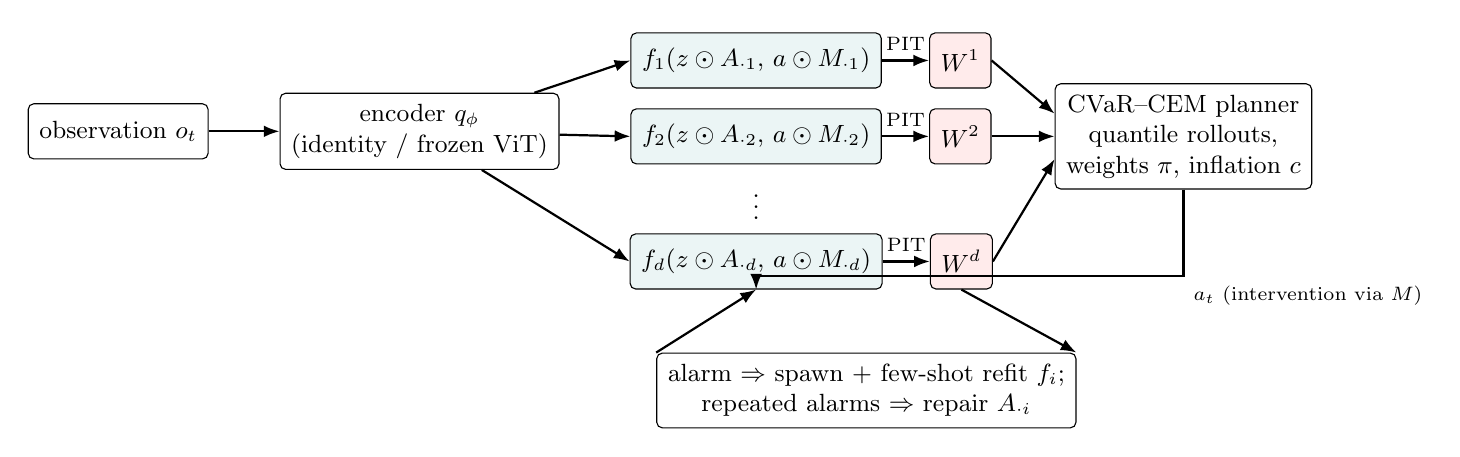
\begin{tikzpicture}[
  font=\small,
  box/.style={draw, rounded corners=2pt, minimum height=7mm,
    inner sep=4pt, align=center},
  mech/.style={box, fill=teal!8},
  gate/.style={box, fill=red!8},
  arr/.style={-{Latex[length=2mm]}, thick},
  node distance=5mm and 9mm]
\node[box] (obs) {observation $o_t$};
\node[box, right=of obs] (enc) {encoder $q_\phi$\\(identity / frozen ViT)};
\node[mech, right=of enc, yshift=9mm] (f1) {$f_1(z\odot A_{\cdot1},\,a\odot M_{\cdot1})$};
\node[mech, below=2.5mm of f1] (f2) {$f_2(z\odot A_{\cdot2},\,a\odot M_{\cdot2})$};
\node[below=0.5mm of f2] (dots) {$\vdots$};
\node[mech, below=0.5mm of dots] (fd) {$f_d(z\odot A_{\cdot d},\,a\odot M_{\cdot d})$};
\node[gate, right=6mm of f1] (g1) {$W^1$};
\node[gate, right=6mm of f2] (g2) {$W^2$};
\node[gate, right=6mm of fd] (gd) {$W^d$};
\node[box, right=8mm of g2, align=center] (plan)
  {CVaR--CEM planner\\quantile rollouts,\\weights $\pi$, inflation $c$};
\node[box, below=8mm of fd, xshift=14mm] (adapt)
  {alarm $\Rightarrow$ spawn + few-shot refit $f_i$;\\
   repeated alarms $\Rightarrow$ repair $A_{\cdot i}$};
\draw[arr] (obs) -- (enc);
\draw[arr] (enc) -- (f1.west);
\draw[arr] (enc) -- (f2.west);
\draw[arr] (enc) -- (fd.west);
\draw[arr] (f1) -- node[above,font=\scriptsize]{PIT} (g1);
\draw[arr] (f2) -- node[above,font=\scriptsize]{PIT} (g2);
\draw[arr] (fd) -- node[above,font=\scriptsize]{PIT} (gd);
\draw[arr] (g1.east) -- (plan.170);
\draw[arr] (g2.east) -- (plan.180);
\draw[arr] (gd.east) -- (plan.190);
\draw[arr] (plan.south) |- node[below right, font=\scriptsize]{$a_t$
(intervention via $M$)} ++(-1.2,-1.1) -| (fd.south);
\draw[arr] (gd.south) -- (adapt.north east);
\draw[arr] (adapt.north west) -- (fd.south);
\end{tikzpicture}}%
\caption{CAIRN architecture. Observations are encoded into a factored
latent state; each variable's mechanism sees only its masked parents and
action targets and outputs quantiles. Each mechanism's PIT residuals feed
its own betting wealth $W^i$, which weights the mechanism library, inflates
rollout uncertainty, and---upon anytime-valid alarms---triggers localized
refits and structure repair. The planner acts through quantile rollouts
and thus routes around unhealthy mechanisms.}\label{fig:flow}
\end{figure}

\section{Experimental evaluation}\label{sec:experiments}

\subsection{Benchmark, baselines, and protocol}

Because the claims concern detection, localization, and adaptation
relative to a known ground truth, the primary testbed is a synthetic
nonlinear dynamic Bayesian network in the spirit of the diagnostic role
that CausalWorld plays for robotic setups \citep{ahmed2021causalworld}:
$d=8$ variables, $m=3$ action coordinates, mechanisms
$z^i_{t+1}=\rho_i z^i_t+\tanh(w_i^\top z_t^{\mathrm{pa}(i)}
+c_i^\top a_t^{\mathrm{tg}(i)}+b_i)+\sigma\xi$ with edge weights bounded
away from zero, known adjacency and action targets, scriptable per-regime
mechanism shifts, and do-interventions on individual variables
(Figure~\ref{fig:graph}). Training data span four regimes (nominal plus
three sparse shifts) with labeled interventions restricted to variables
$\{0,1,2,3\}$, so that do-queries on the remaining variables are
compositionally held out. We compare against a monolithic quantile world
model of matched training budget (the canonical
DreamerV3/TD-MPC2-style commitment, in state space), a five-member
probabilistic ensemble with trajectory sampling \citep{chua2018deep}, an
oracle-tuned per-variable CUSUM detector, a global e-gate over the
monolithic model (isolating why localization requires structure), and
CAIRN ablations (oracle graph; no invariance term). All experiments run
on CPU; the complete suite trains in under an hour.

\begin{figure}[t]
\centering
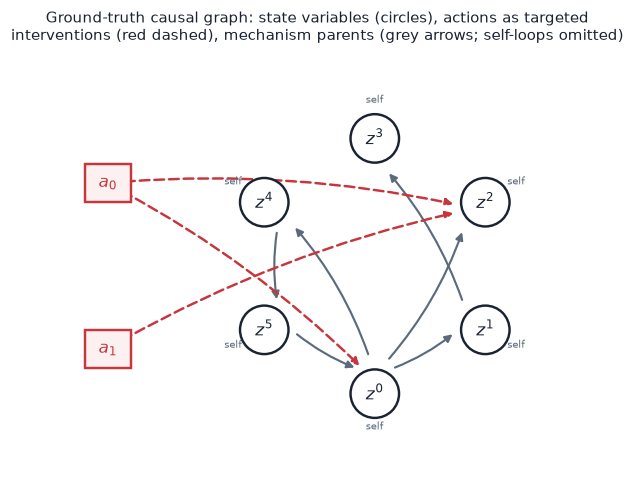
\includegraphics[width=0.62\textwidth]{figures/fig_graph.png}
\caption{A six-variable instance of the ground-truth benchmark family
used for illustration throughout: state variables (circles) with sparse
parent edges (grey), and action coordinates entering as targeted
interventions (dashed). The evaluation suite uses $d=8$ variables with
in-degree two.}\label{fig:graph}
\end{figure}

\subsection{Detection and localization (RQ2)}\label{sec:rq2}

Table~\ref{tab:rq2} contains the headline result.
Figure~\ref{fig:egate} shows a representative episode. Across ten
unannounced shift scenarios (eight single-mechanism sign flips and two
two-mechanism shifts), the e-gates detect the shifted mechanisms with a
median delay of eighteen steps and localize them with a mean $F_1$ of
$0.97$; over three $6{,}000$-step stationary null streams they raise
\emph{zero} false alarms, consistent with (and conservatively below) the
guarantee of Proposition~\ref{prop:validity}, which the exact-null
verification confirms independently at an alarm fraction of $0.0000$.
The comparison detectors illustrate both classical failure modes.
Oracle-tuned CUSUM is sometimes instantaneous but wildly inconsistent:
its thresholds, tuned to zero false alarms on one null stream, produce a
$0.42$ per-gate false-alarm fraction on fresh null streams, and its
localization $F_1$ of $0.68$ mixes perfect scenarios with complete
misses. Ensemble disagreement fires quickly but names the wrong
variables ($F_1=0.28$) and false-alarms on half the gates. The global
e-gate on the monolithic model---the ablation that removes
structure---detects the same shifts but nine times slower (median
$159$ steps, since the evidence of one broken mechanism is diluted
across the whole model) and cannot localize by construction.

\begin{figure}[t]
\centering
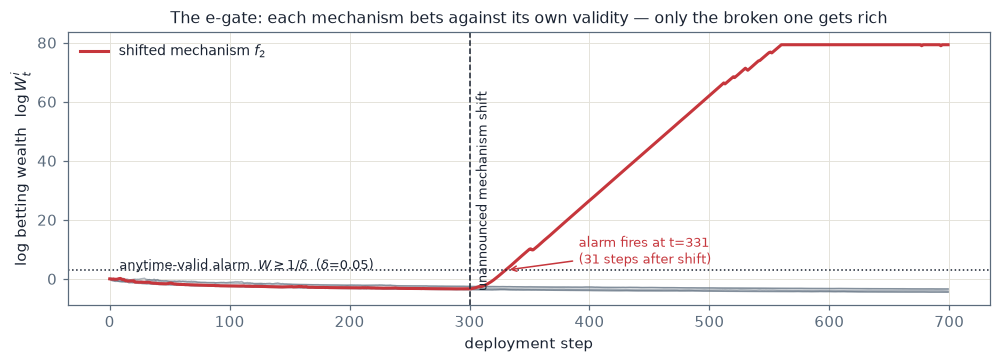
\includegraphics[width=\textwidth]{figures/fig_egate.png}
\caption{The e-gate catching a broken mechanism. At step 300 one
mechanism's dynamics are silently sign-flipped. Healthy mechanisms' log
wealth stays near zero (grey); the broken mechanism's wealth grows
exponentially and crosses the anytime-valid threshold 31 steps later. The
alarm names exactly the variable whose physics changed.}
\label{fig:egate}
\end{figure}

\begin{table}[t]
\caption{Detection and localization (RQ2), aggregated over ten unannounced
mechanism-shift scenarios and three $6{,}000$-step stationary null streams
at level $\delta=0.05$. The e-gates run with no tuning; CUSUM and ensemble
thresholds receive oracle tuning on a separate null stream. The exact-null
verification (gates fed probability integral transforms from the true
environment conditional) produced an alarm fraction of
$0.0000$, consistent with
Proposition~\ref{prop:validity}. $^{\ast}$per stream rather than per gate.}
\label{tab:rq2}
\small\setlength{\tabcolsep}{4pt}%
\begin{tabular}{lccccc}
\toprule
Detector & Null alarms & Med.\ delay & Loc.\ $F_1$ & Prec.\ & Rec.\\
\midrule
CAIRN e-gates & 0.000 & 18 & 0.967 & 0.950 & 1.000 \\
e-gates, oracle graph & 0.000 & 25 & 0.967 & 0.950 & 1.000 \\
CUSUM & 0.417 & 2 & 0.680 & 0.617 & 0.800 \\
Ensemble disagreement & 0.500 & 20 & 0.284 & 0.237 & 0.700 \\
Global e-gate (monolithic) & 0.667$^{\ast}$ & 159 & \multicolumn{3}{c}{undefined (no localization)} \\
\botrule
\end{tabular}
\end{table}


\subsection{Interventional generalization (RQ1)}

Table~\ref{tab:rq1} evaluates off-support do-queries
($\dt(z^i{=}\pm4)$, far outside the reachable range) on held-out and
trained do-targets. The structural signature is unambiguous: with the
oracle graph, non-descendant error under intervention \emph{equals} the
no-intervention reference to three decimals, as
Proposition-level reasoning predicts and Figure~\ref{fig:surgery}
visualizes; the learned graph leaks almost nothing (e.g.\ $0.580$ against
a reference of $0.552$ on trained targets); the monolithic model leaks
severely ($0.708$ against $0.456$, a $55\%$ violation), and the ensemble
similarly. On raw rollout RMSE, by contrast, all model classes are
statistically tied at long horizons: in this stochastic, multi-attractor
environment, long-horizon error is dominated by attractor-branching
uncertainty that afflicts every model equally. We report this honestly
rather than claiming a rollout-accuracy advantage; the causal
factorization buys \emph{invariance} and everything built on it
(localization, adaptation, honest uncertainty), not a smaller
mean-squared error on this benchmark.

\begin{table}[t]
\caption{Interventional generalization (RQ1). Rollout RMSE of the
model-mean trajectory against the true conditional mean under off-support
do-interventions ($\mathrm{do}(z^i{=}\pm 4)$), for do-targets never
intervened during training (held-out) and for trained do-targets, together
with the structural split at horizon $3$: error on descendants versus
non-descendants of the intervened variable, and the no-intervention
reference error of the same non-descendant set. A structurally correct
model must leave non-descendants unchanged, so its non-descendant column
must match the reference column.}\label{tab:rq1}
\small\setlength{\tabcolsep}{3.5pt}%
\begin{tabular}{llcccccc}
\toprule
Targets & Model & $h{=}1$ & $h{=}3$ & $h{=}5$ & desc.\ & non-desc.\ & ref.\\
\midrule
held-out & CAIRN (learned graph) & 0.349 & 1.025 & 1.748 & 0.657 & 0.758 & 0.739 \\
held-out & CAIRN w/o $\mathcal{L}^{\mathrm{inv}}$ & 0.376 & 1.065 & 1.791 & 0.649 & 0.809 & 0.815 \\
held-out & CAIRN (oracle graph) & 0.412 & 1.017 & 1.640 & 0.616 & 0.744 & 0.744 \\
held-out & Monolithic WM & 0.328 & 0.916 & 1.524 & 0.607 & 0.757 & 0.726 \\
held-out & Probabilistic ensemble & 0.346 & 1.017 & 1.715 & 0.759 & 0.790 & 0.745 \\
\midrule
trained & CAIRN (learned graph) & 0.313 & 0.990 & 1.405 & 0.885 & 0.580 & 0.552 \\
trained & CAIRN w/o $\mathcal{L}^{\mathrm{inv}}$ & 0.342 & 1.003 & 1.445 & 0.912 & 0.595 & 0.605 \\
trained & CAIRN (oracle graph) & 0.379 & 0.998 & 1.403 & 0.704 & 0.671 & 0.671 \\
trained & Monolithic WM & 0.276 & 1.105 & 1.594 & 1.043 & 0.708 & 0.456 \\
trained & Probabilistic ensemble & 0.288 & 1.061 & 1.521 & 1.089 & 0.616 & 0.476 \\
\botrule
\end{tabular}
\end{table}


\subsection{Localized adaptation (RQ3)}

Table~\ref{tab:rq3} compares evidence-triggered localized refits against
full fine-tuning of either CAIRN or the monolithic model at a matched
gradient budget on the same post-shift stream. The localized refit
improves the shifted mechanisms steadily while the error of the seven
healthy mechanisms is untouched---overall error \emph{decreases}
throughout adaptation. Both fine-tuning baselines suffer catastrophic
interference: mid-adaptation, the monolithic model's overall error is
an order of magnitude above its pre-shift level, and after four hundred
samples it remains several times worse than before the shift. No method
reaches the strict pre-shift error level within the window---the refit
window of 96 samples bounds the achievable fit---which we report as a
limitation of few-shot refitting rather than hiding it in a favorable
metric.

\begin{table}[t]
\caption{Localized adaptation versus fine-tuning (RQ3): one-step median
RMSE after an unannounced shift of mechanism set $S$, as a function of the
number of post-shift samples $n$, evaluated on the shifted variables
(``shifted'') and on all variables (``all''). All methods receive the same
stream and the same gradient budget. Full fine-tuning suffers catastrophic
interference on the seven healthy mechanisms; the evidence-triggered
localized refit leaves them untouched.}\label{tab:rq3}
\footnotesize\setlength{\tabcolsep}{2.5pt}%
\begin{tabular}{lllcccccc}
\toprule
Shift & Method & Nodes & $n{=}0$ & $n{=}25$ & $n{=}50$ & $n{=}100$ & $n{=}200$ & $n{=}400$\\
\midrule
$S{=}\{1\}$ & CAIRN localized refit & shifted & 0.819 & 0.819 & 0.541 & 0.541 & 0.358 & 0.360 \\
 &  & all & 0.347 & 0.347 & 0.270 & 0.270 & 0.229 & 0.229 \\
$S{=}\{1\}$ & CAIRN full fine-tune & shifted & 0.819 & 0.489 & 0.459 & 0.435 & 0.327 & 0.256 \\
 &  & all & 0.347 & 1.899 & 2.497 & 2.824 & 0.770 & 0.681 \\
$S{=}\{1\}$ & Monolithic fine-tune & shifted & 0.743 & 0.972 & 5.026 & 4.656 & 0.693 & 0.694 \\
 &  & all & 0.332 & 1.456 & 3.310 & 3.176 & 0.967 & 1.163 \\
\midrule
$S{=}\{3,5\}$ & CAIRN localized refit & shifted & 1.495 & 1.572 & 1.571 & 1.304 & 1.312 & 0.449 \\
 &  & all & 0.771 & 0.809 & 0.808 & 0.793 & 0.802 & 0.331 \\
$S{=}\{3,5\}$ & CAIRN full fine-tune & shifted & 1.495 & 0.576 & 2.584 & 2.152 & 1.318 & 1.460 \\
 &  & all & 0.771 & 0.828 & 1.552 & 1.915 & 1.622 & 1.039 \\
$S{=}\{3,5\}$ & Monolithic fine-tune & shifted & 1.460 & 1.495 & 1.179 & 1.413 & 2.108 & 2.330 \\
 &  & all & 0.802 & 1.343 & 2.507 & 2.936 & 2.396 & 2.260 \\
\bottomrule
\end{tabular}
\end{table}


\subsection{Calibration (RQ4)}

Table~\ref{tab:rq4} reports empirical coverage of nominal $90\%$ rollout
intervals. In distribution, CAIRN's intervals are near-nominal across
horizons where the ensemble under-covers. Under an unannounced shift and
before any adaptation, the stale intervals lose coverage on the shifted
variable; evidence-driven inflation \eqref{eq:inflation} restores
honesty precisely there, at the cost of width, and after localized
adaptation coverage returns without inflation doing the work
(Figure~\ref{fig:inflation}). This is the operational meaning of
``knowing where the imagined future is untrustworthy''.

\begin{figure}[t]
\centering
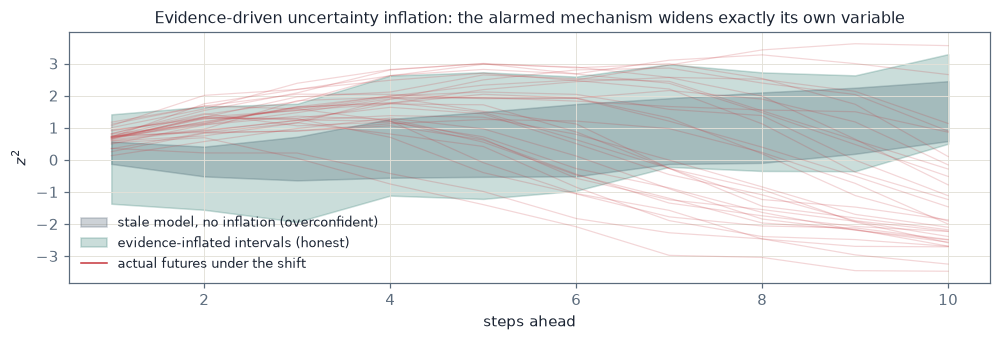
\includegraphics[width=\textwidth]{figures/fig_inflation.png}
\caption{Evidence-driven uncertainty inflation on the shifted variable.
The stale mechanism's old intervals (grey) miss the actual post-shift
futures (thin lines); inflating the spread of exactly the alarmed
mechanism (shaded, capped by \eqref{eq:inflation}) restores honest
coverage without touching healthy variables.}\label{fig:inflation}
\end{figure}

\begin{table}[t]
\caption{Calibration (RQ4): empirical coverage of nominal $90\%$ rollout
intervals by horizon. In-distribution rows average over all variables;
shift rows are scored on the shifted mechanism's variable when available
(all-node averages otherwise), where interval honesty is actually at
stake.}\label{tab:rq4}
\begin{tabular}{llcccc}
\toprule
Condition & Scope & $h{=}1$ & $h{=}5$ & $h{=}10$ & $h{=}15$\\
\midrule
in-distribution & CAIRN (learned graph) & 0.964 & 0.947 & 0.927 & 0.941 \\
in-distribution & Probabilistic ensemble & 0.880 & 0.841 & 0.859 & 0.879 \\
\midrule
shift, stale intervals & all nodes & 0.880 & 0.848 & 0.896 & 0.868 \\
shift, evidence-inflated & all nodes & 0.924 & 0.911 & 0.935 & 0.928 \\
shift, ensemble & all nodes & 0.806 & 0.759 & 0.823 & 0.785 \\
shift, after adaptation & all nodes & 0.923 & 0.928 & 0.892 & 0.900 \\
\botrule
\end{tabular}
\end{table}


\subsection{Structure recovery and regime diversity (RQ6)}

Table~\ref{tab:rq6} shows recovery of $A$ and $M$ as the number of
training regimes grows, holding the total number of episodes fixed.
Action-target recovery improves markedly with regime diversity ($F_1$
from $0.57$ with a single regime to $0.89$ with four or more), in line
with the identifiability role of interventional variation
\citep{ahuja2023interventional}; adjacency recovery is high throughout,
with residual errors concentrated on edges whose influence approaches
the noise floor. Downstream planning (RQ5) shows parity with the
monolithic baseline in the nominal regime and a directional advantage
for the adapted model after shifts, but with only six evaluation
episodes per condition the intervals are wide, and we treat these
planning numbers as preliminary.

\begin{table}[t]
\caption{Structure recovery versus regime diversity (RQ6): structural
Hamming distance and edge $F_1$ of the learned adjacency $A$ and
action-target mask $M$ against ground truth, as the number of training
regimes grows.}\label{tab:rq6}
\begin{tabular}{ccccc}
\toprule
Regimes & SHD$(A)$ & $F_1(A)$ & SHD$(M)$ & $F_1(M)$\\
\midrule
1 & 4 & 0.889 & 3 & 0.571 \\
2 & 4 & 0.889 & 3 & 0.571 \\
4 & 8 & 0.800 & 1 & 0.889 \\
6 & 6 & 0.842 & 1 & 0.889 \\
\botrule
\end{tabular}
\end{table}


\section{Conclusion}\label{sec:conclusion}

We introduced CAIRN, a world model that couples a causally factored
transition kernel with per-mechanism anytime-valid betting martingales,
and showed that the joint construction produces a qualitatively new
capability: a model that degrades \emph{locally and detectably} under
mechanism shifts instead of globally and silently. The e-gate's
guarantees are simple, tuning-free, and---with conformal PIT
recalibration and a tolerance null---hold for learned mechanisms rather
than only in theory; on the ground-truth benchmark the gates achieved
zero false alarms while localizing real shifts within tens of steps,
where oracle-tuned classical detectors and ensembles fail in one
direction or the other. Evidence-triggered adaptation repaired exactly
the broken mechanisms without interference, and evidence-proportional
inflation kept imagined futures honest while stale.

Several limitations bound these claims, and we state them together with
the conclusions they qualify. The primary instantiation is in state
space; pixel-based instantiations are architecturally prepared through a
frozen visual encoder, but not yet evaluated. The tolerance null makes
approximation error unflaggable below $\varepsilon$ by design, and the
sliding-holdout maintenance that keeps healthy gates quiet can absorb
drifts below the tolerance; both are the operationally correct
compromise, and both are stated on the tin. On raw long-horizon rollout
accuracy the causal factorization brought no advantage in our
multi-attractor benchmark, and the planning gains after adaptation,
while directionally consistent, need many more evaluation episodes.
Finally, all reported numbers come from a single benchmark seed;
multi-seed confidence intervals, the robotic instantiations on
CausalWorld and the DeepMind Control suite
\citep{ahmed2021causalworld,tassa2018deepmind}, offline PIT-validity
evaluation on real robot trajectories from DROID
\citep{khazatsky2024droid}, and the financial-network instantiation in
which do-queries answer contagion questions
\citep{eisenberg2001systemic,battiston2012debtrank} are the immediate
next steps of this program.

\ifanon\else
\section*{Data availability}
The complete implementation, the ground-truth benchmark, all experiment
scripts, result files, and the scripts that regenerate every table of
this paper are available at
\url{https://github.com/vinhqdang/CAIRN-A-Causally-Factored-Self-Certifying-World-Model-for-Interventional-Generalization}.
\fi
\ifanon
\section*{Data availability}
The complete implementation, the ground-truth benchmark, all experiment
scripts, result files, and the scripts that regenerate every table of
this paper will be released in a public repository upon acceptance; an
anonymized archive is provided to reviewers.
\fi

\bibliography{references}

\end{document}
